
\section{Oplossen van vergelijkingen}

Het vullen van vierkanten, kubussen en $n$-dimensionale kubussen kan heel origineel gebruikt worden om vergelijkingen op te lossen. 

\subsection{Oplossen van vierkantsvergelijkingen}

Een {\bf vierkantsvergelijking} is een vergelijking van de vorm $ax^2 + bx + c = 0$. Dus de hoogste graad van de onbekende is $2$. Je hebt reeds methoden gezien om vergelijkingen van deze vorm op te lossen. De typische methoden zijn
\begin{itemize}
  \item Merkwaardige producten gebruiken.
  \item Ontbinden in factoren door delers te zoeken.
  \item Gebruik maken van de som en product.
  \item De formule met behulp van discriminant.
\end{itemize}

\ask{Welke van de bovenstaande methoden kennen jullie reeds?}

\answer[1cm]{}

\subsubsection{Een eenvoudig geval}

Een heel eenvoudige vierkantsvergelijking is
$$
x^2+2x+1=0\;.
$$

\ask{Wat is de eenvoudigste methode die je kan gebruiken? Los deze vierkantsvergelijking ook op.}

\answer[3cm]{We kunnen een merkwaardig product gebruiken om de veelterm te ontbinden in factoren: $x^2+2x+1=(x+1)^2$ Nadien kunnen we de oplossingen aflezen. De vergelijking heeft als oplossing twee keer $-1$, dus de oplossingsverzameling is $Opl=\{-1\}$.}

We zullen hier nu nog een methode voor het oplossen van een vierkantsvergelijking aan toevoegen. Dit door een vierkant te construeren met kleinere vierkanten en rechthoeken. Hiervoor zullen we de kwadratische term en de constante term zien als een vierkant, de andere getallen zullen we zien als rechthoeken. In ons bovenstaand voorbeeld hebben we $x^2$ en $1$. We construeren twee vierkanten:

\begin{center}
\begin{tikzpicture}[scale=0.5, line cap=round,line join=round,>=triangle 45,x=1.0cm,y=1.0cm]
\clip(-1,-1) rectangle (9,6);
\filldraw[line width=1.6pt,fill=black,fill opacity=0.1] (0,0) -- (5,0) -- (5,5) -- (0,5) -- cycle;
\filldraw[line width=1.6pt,fill=black,fill opacity=0.1] (7,0) -- (8,0) -- (8,1) -- (7,1) -- cycle;
\draw (2,0) node[anchor=north west] {$x$};
\draw (-1,2.87) node[anchor=north west] {$x$};
\draw (7,0) node[anchor=north west] {$1$};
\draw (6,1) node[anchor=north west] {$1$};
\end{tikzpicture}

\end{center}

We hebben nog $2x$ over. Dit moeten we zien als een rechthoek. Een rechthoek van grootte $2$ bij $x$ helpt ons niets, want dan hebben we twee vierkanten en \'e\'en rechthoek die we niet kunnen samenvoegen om \'e\'en vierkant mee op te vullen. We zullen dus de overige $2x$ opsplitsen in $x + x$. Hiervan maken we dan twee rechthoeken met grootte $1$ bij $x$:

\begin{center}
\begin{tikzpicture}[scale=0.5, line cap=round,line join=round,>=triangle 45,x=1.0cm,y=1.0cm]
\clip(-1,-1) rectangle (5,6);
\filldraw[line width=1.6pt,fill=black,fill opacity=0.1] (0,0) -- (1,0) -- (1,5) -- (0,5) -- cycle;
\filldraw[line width=1.6pt,fill=black,fill opacity=0.1] (3,0) -- (4,0) -- (4,5) -- (3,5) -- cycle;
\draw (2,2.8) node[anchor=north west] {$x$};
\draw (-1,2.8) node[anchor=north west] {$x$};
\draw (0,0) node[anchor=north west] {$1$};
\draw (3,0) node[anchor=north west] {$1$};
\end{tikzpicture}

\end{center}

Nu zou het mogelijk moeten zijn om de figuren te verschuiven en te roteren zodanig dat je met de vier figuren \'e\'en groter vierkant kunt maken.

\task{Puzzel nu met de vier figuren tot je \'e\'en groter vierkant hebt. Desnoods kan je de figuren uitknippen uit een apart blad papier om hiermee te puzzelen. Teken hieronder dan het resultaat.}

\answer[5cm]{
\begin{center}
\begin{tikzpicture}[scale=0.5, line cap=round,line join=round,>=triangle 45,x=1.0cm,y=1.0cm]
\clip(-1,-1) rectangle (7,7);
\filldraw[line width=1.6pt,fill=black,fill opacity=0.1] (0,0) -- (5,0) -- (5,5) -- (0,5) -- cycle;
\filldraw[line width=1.6pt,fill=black,fill opacity=0.1] (5,0) -- (6,0) -- (6,5) -- (5,5) -- cycle;
\filldraw[line width=1.6pt,fill=black,fill opacity=0.1] (5,5) -- (6,5) -- (6,6) -- (5,6) -- cycle;
\filldraw[line width=1.6pt,fill=black,fill opacity=0.1] (0,5) -- (5,5) -- (5,6) -- (0,6) -- cycle;
\draw (2,0) node[anchor=north west] {$x$};
\draw (-1,2.8) node[anchor=north west] {$x$};
\draw (5,0) node[anchor=north west] {$1$};
\draw (-1,6) node[anchor=north west] {$1$};
\end{tikzpicture}

\end{center}
}

\ask{Wat is nu de oppervlakte van het bekomen vierkant? Kan je hiermee de vergelijking oplossen?}

\answer[3cm]{De oppervlakte is $(x+1)^2$. De oplossing is dan $Opl=\{-1\}$.}

Je kan analoog redeneren om de oplossingen te zoeken van elke vergelijking van de vorm $a^2x^2+2abx+b^2=0$. 

\subsubsection{Een iets moeilijkere vergelijking}

We beginnen opnieuw met een vergelijking die mag opgelost worden met \'e\'en van de gekende methoden. Neem als vergelijking
$$
x^2+4x-5=0\;.
$$

Opnieuw zien we $x^2$ als een vierkant met zijde $x$. Ook zien we $4x$ terug als twee rechthoeken, beide met de zijden $x$ en $2$. We hebben dan al $x^2+4x=x^2+2x+2x$ waarbij de volgende figuur hoort.
\begin{center}
\begin{tikzpicture}[scale=0.5, line cap=round,line join=round,>=triangle 45,x=1.0cm,y=1.0cm]
\clip(-1,-1) rectangle (8,8);
\filldraw[line width=1.6pt,fill=black,fill opacity=0.1] (0,0) -- (5,0) -- (5,5) -- (0,5) -- cycle;
\filldraw[line width=1.6pt,fill=black,fill opacity=0.1] (5,0) -- (7,0) -- (7,5) -- (5,5) -- cycle;
\filldraw[line width=1.6pt,fill=black,fill opacity=0.1] (0,5) -- (5,5) -- (5,7) -- (0,7) -- cycle;
\draw (2.56,0) node[anchor=north] {$x$};
\draw (-0.5,2.87) node[anchor=north] {$x$};
\draw (6,0) node[anchor=north] {$2$};
\draw (-0.5,6.5) node[anchor=north] {$2$};
\end{tikzpicture}

\end{center}

Uit de vergelijking weten we dat $x^2+4x=5$. Dus de oppervlakte van deze figuur moet gelijk zijn aan $5$! Laten we deze figuur eens vervolledigen door rechtsboven een klein vierkantje van $2$ bij $2$ aan toe te voegen:

\begin{center}
\begin{tikzpicture}[scale=0.5, line cap=round,line join=round,>=triangle 45,x=1.0cm,y=1.0cm]
\clip(-1,-1) rectangle (8,8);
\filldraw[line width=1.6pt,fill=black,fill opacity=0.1] (0,0) -- (5,0) -- (5,5) -- (0,5) -- cycle;
\filldraw[line width=1.6pt,fill=black,fill opacity=0.1] (5,0) -- (7,0) -- (7,5) -- (5,5) -- cycle;
\filldraw[line width=1.6pt,fill=black,fill opacity=0.1] (0,5) -- (5,5) -- (5,7) -- (0,7) -- cycle;
\filldraw[line width=1.6pt,fill=black,fill opacity=0.1] (5,5) -- (7,5) -- (7,7) -- (5,7) -- cycle;
\draw (2.56,0) node[anchor=north] {$x$};
\draw (-0.5,2.87) node[anchor=north] {$x$};
\draw (6,0) node[anchor=north] {$2$};
\draw (-0.5,6.5) node[anchor=north] {$2$};
\end{tikzpicture}

\end{center}

De oppervlakte van deze nieuwe figuur is dus de oppervlakte van de vorige figuur plus de oppervlakte van het nieuwe vierkantje van $2$ bij $2$. De oppervlakte is dus $5 + 4 = 9$. De lengte van de zijde van dit vierkant is dus $\sqrt{9}=3$. Maar we wisten ook reeds dat de lengte van deze figuur $x+2$ was. We leiden dus gemakkelijk de waarde voor $x$ af.

\ask{Stel beide manieren om de lengte van de zijde te berekenen aan elkaar gelijk en los daar dan $x$ uit op.}

\answer[3cm]{
\begin{align*}
  3 &= x + 2\\
  \Leftrightarrow\quad 3-2 &= x\\
  \Leftrightarrow\quad x&=1
\end{align*}
}

We zien dat we in de figuur het vierkant $x^2$ te groot hebben getekend ten opzicht van de rechthoek van $x$ bij $2$ maar dat is niet erg. Het was maar een schets.

\task{De vergelijking $x^2+4x-5=0$ heeft nog een tweede oplossing. Bepaal deze met een methode die je reeds kent (hint: aangezien $x=1$ een oplossing is, heb je reeds de deler $(x-1)$ van de veelterm $x^2+4x-5$ gevonden.) Waarom denk je dat het niet mogelijk is om door het vullen van een vierkant de andere oplossing te vinden?}

\answer[4cm]{We berekenen het quoti\"ent van $x^2+4x-5$ en $x-1$. We zien dat dit $x+5$ is. De andere oplossing voor $x$ is dus $-5$. Omdat negatieve getallen geen lengte voor kunnen stellen kan hiermee dan ook geen vierkant geconstrueerd worden.}

\subsubsection{Een algemenere methode}

Bekijk nu eens de volgende vergelijking
$$
x^2-8x-20 = 0\;.
$$

\ask{Is het mogelijk om dezelfde techniek als voordien toe te passen? Waarom niet?}

\answer[3cm]{Neen. We kunnen geen rechthoeken construeren want de co\"effici\"ent bij de term van de eerste graad is negatief.}

\ask{Heb je een idee hoe je dit probleem zou kunnen verhelpen?}

Volg nu mee om deze vergelijking toch op te lossen.

\task{Teken een vierkant met zijde $x$.}

\answer[4cm]{
\begin{center}
\begin{tikzpicture}[scale=0.3, line cap=round,line join=round,>=triangle 45,x=1.0cm,y=1.0cm]
\clip(-1,-1) rectangle (11,11);
\filldraw[line width=1.6pt,fill=black,fill opacity=0.1] (0,0) -- (10,0) -- (10,10) -- (0,10) -- cycle;
\draw (5,0.25) node[anchor=north] {$x$};
\draw (-0.75,5) node[anchor=north] {$x$};
\end{tikzpicture}

\end{center}
}

Dit vierkant zal dus een oppervlakte van $x^2$ hebben.

\task{Teken nu in het vierkant van daarnet twee rechthoeken van 4 bij x. Deze moeten \uline{binnen in} het vierkant zelf getekend worden, bijvoorbeeld \'e\'en bovenaan, en \'e\'en rechts.}

\answer[4cm]{
\begin{center}
\begin{tikzpicture}[scale=0.3, line cap=round,line join=round,>=triangle 45,x=1.0cm,y=1.0cm]
\clip(-1,-1) rectangle (11,11);
\filldraw[line width=1.6pt,fill=black,fill opacity=0.1] (0,0) -- (10,0) -- (10,10) -- (0,10) -- cycle;
\filldraw[line width=1.6pt,fill=black,fill opacity=0.1] (6,0) -- (10,0) -- (10,10) -- (6,10) -- cycle;
\filldraw[line width=1.6pt,fill=black,fill opacity=0.1] (0,6) -- (10,6) -- (10,10) -- (0,10) -- cycle;
\draw (5,0.25) node[anchor=north] {$x$};
\draw (-0.75,5) node[anchor=north] {$x$};
\draw (8,1.75) node[anchor=north] {$4$};
\draw (1,8.5) node[anchor=north] {$4$};
\end{tikzpicture}

\end{center}
}

\ask{De twee rechthoeken overlappen elkaar. Wat is de oppervlakte van het overlappend stukje?}

\answer[1cm]{$4\cdot 4=16$.}

Linksonder blijft dan nog een stukje met oppervlakte $(x-4)^2$ over. Uit de figuur weten we dat dit gelijk is aan $x^2 -4x -4x$ plus het overlappend deel met oppervlakte $16$. En uit de vergelijking weet je dat $x^2 -4x -4x=20$ is.

\task{Stel beide manieren om de oppervlakte van het kleine vierkantje linksonder te berekenen aan elkaar gelijk en haal er zo een oplossing voor $x$ uit.}

\answer[3cm]{
\begin{align*}
  (x-4)^2 &= x^2 -4x -4x + 16\\
          &= 20 +16\\
          &= 36\\
\end{align*}
We kunnen nu de positieve wortel nemen want afstanden zijn positief, we krijgen dan
$$ x-4 = 6\;.$$
We vinden dus een oplossing $x=10$. De andere oplossing kan bepaald worden door de tweedegraadsveelterm $x^2-8x-20$ te delen door $x-10$.
} 

Zo zie je maar. Een probleem uit de algebra kan gerust opgelost worden met een beetje meetkunde! Deze methode voor het oplossen van vierkantsvergelijkingen gebruikt het idee van kwadraatafsplitsen en werd voor het eerst gebruikt door Al-Khwarizmi. Deze werd geboren in Uzbekistan rond 780. Hij schreef verscheidene boeken over wiskunde waaronder een invloedrijk boek over eerste- en tweedegraadsvergelijkingen. Hierin werd alles dus op een meetkundige manier beschreven, zoals ook wij daarnet deden.

\subsection{Oplossen van derdegraadsvergelijkingen}

\begin{wrapfigure}[9]{r}{0.2\textwidth}
  \centering
  \vspace*{-0.5cm}
  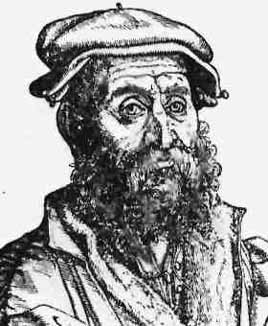
\includegraphics[width=0.2\textwidth]{Tartaglia}\\
  Tartaglia
\end{wrapfigure}

Net zoals we vierkantsvergelijkingen meetkundig kunnen oplossen met behulp van een vierkant, kunnen we dit uitbreiden voor derdegraadsvergelijkingen. De ontdekking van een methode om algemeen derdegraadsvergelijkingen op te lossen steunt op het vullen van een kubus! Hiervoor moeten we terug gaan naar het begin van de 16de eeuw. In Bologna was een universiteit waar wiskundigen uit gans Europa verzamelden. Daar waren wiskunde wedstrijden met toeschouwers populair! De wiskundigen daagden elkaar uit om in zo weinig mogelijk tijd bepaalde problemen op te lossen. Men geloofde echter dat het oplossen van derdegraadsvergelijkingen onmogelijk was.

De Italiaan Tartaglia zou aantonen dat iedereen ongelijk had. Tartaglia wat staat voor de stotteraar was de bijnaam van Niccolo Fontanas. Als twaalfjarig kind werd hij verminkt in het gezicht door een Franse soldaat. Het resultaat was een groot en lelijk litteken en een spraakgebrek. Zijn leeftijdsgenoten negeerden hem. Reden om als kind diep ongelukkig te zijn. Gelukkig voor de jonge Tartaglian vond hij in de wiskunde een wereld vol uitdagingen. Het duurde dan ook niet lang voordat hij een methode vond om een welbepaalde vorm van derdegraadsvergelijkingen op te lossen.

Ook een andere jonge wiskundige beweerde dat hij ook derdegraadsvergelijkingen kon oplossen. Wanneer de ontdekkingen algemeen bekend werden organiseerde men maar al te graag een wedstrijd om beide jongeren tegen elkaar uit te brengen.

Het probleem voor Tartaglia was dat hij maar \'e\'en enkele soort derdegraadsvergelijking kon oplossen. De organisators van de wedstrijd waren natuurlijk van plan om allerlei soorten vergelijkingen van de derde graad te vragen. Maar een paar dagen voor de wedstrijd slaagde Tartaglia erin om toch nog methoden te vinden voor de andere typen derdegraadsvergelijkingen op te lossen. Met deze nieuwe wapens slaagde Tartaglia erin om tijdens de wedstrijd alle vragen op te lossen in minder dan twee uur en zijn tegenstander op verpletterende wijze te verslaan!

\begin{wrapfigure}[9]{l}{0.2\textwidth}
  \centering
  \vspace*{-0.5cm}
  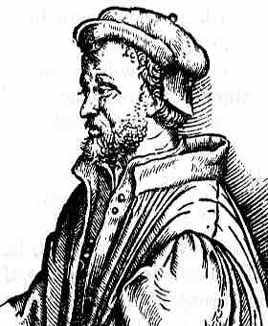
\includegraphics[width=0.2\textwidth]{Cardan}\\
  Cardano
\end{wrapfigure}

Girolamo Cardano, een Milaanse wiskundige, was zo wanhopig op zoek naar de methode om ook derdegraadsvergelijkingen op te lossen dat hij Tartaglia overhaalde om zijn geheim prijs te geven. Tartaglia, gestreeld door de aandacht van Cardano, was bereid zijn geheim prijs te geven onder \'e\'en voorwaarde. Cardano moest het geheim voor zichzelf houden en het nooit publiceren!

Cardano kon het niet laten om de methode te bespreken met zijn briljante student Ferrari. Ferrari, een wiskundige geboren in Bologna, besefte dat hij de methode van Tartaglia kon gebruiken om de nog moeilijkere vergelijkingen van de vierde graad op te lossen. Een roemrijke daad! Cardano kon zijn student Ferrari de erkenning niet weigeren. En die erkenning bij wiskundigen is net publiceren. Omdat het werk van Ferrari steunde op derdegraadsvergelijkingen brak Cardano zijn belofte aan Tartaglia en publiceerden Cardano en Ferrari een artikel over vierdegraadsvergelijkingen.

De methode van Tartaglia, die Cardano in zijn werk Ars Magna beschrijft, wordt ondersteunt door een meetkundige manier van oplossen. Met deze methode kan je bijvoorbeeld de vergelijking \[x^3+6x-20=0\] oplossen. Tartaglia zag bij de vergelijking $x^3-6x-20=0$, $x^3$ als een kubus met ribbe $x$ en dus met een inhoud van $x^3$. Daarnaast stelde hij $6x$ voor als 3 gelijke balken met elk een inhoud van $2x$ en met de lengte ��n zijde gelijk aan $x$, terwijl de ander nog niet vastliggen. De bedoeling was om met die balken terug een kubus te vormen samen met de eerste kubus met inhoud $x^3$. Het plaatste de balken zo aan de kubus zodat hij uiteindelijk bijna een kubus kreeg. Er bleef namelijk nog een kleine kubus over. De vergelijking $x^3+6x-20=0$ geeft aan dat de inhoud van deze laatste kubus gelijk is aan 20. Tartaglia maakt van deze figuur een complete kubus door een kleine kubus toe te voegen zoals in Figuur \ref{fig:kubus}. Door het gelijkstellen van de ribbe van de kleine kubus als $v$ en de ribbe van de grote kubus $u$ en hiermee verder rekenend, kon er dan ��n oplossing gevonden worden, namelijk $x=2$.

\begin{figure}[h]
  \centering
  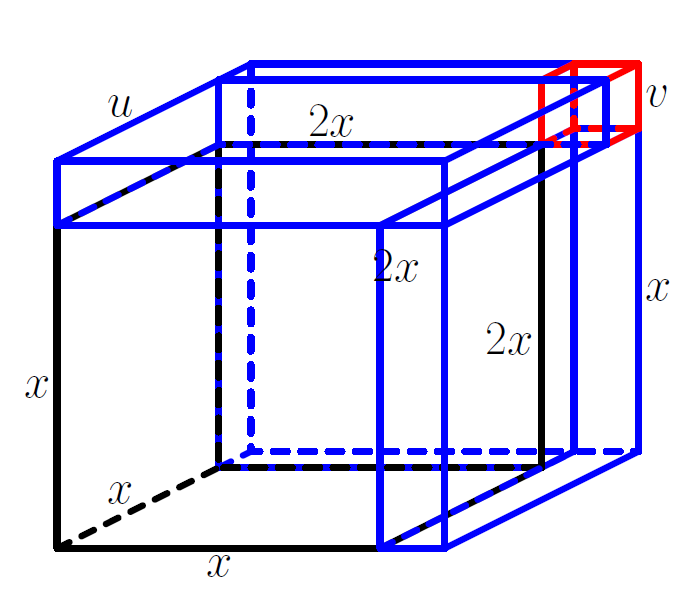
\includegraphics[width=0.4\textwidth]{kubus}
  \caption{Complete kubus gebruikt voor het oplossen van $x^3+6x-20=0$.}
  \label{fig:kubus}
\end{figure}
















